%%%%%%%%%%%%%%%%%%%%%%%%%%%%%%%%%%%%%%%%%%%%%%%%%%%%%%%%%%%%
%%  This Beamer template was created by Cameron Bracken.
%%  Anyone can freely use or modify it for any purpose
%%  without attribution.
%%
%%  Last Modified: January 9, 2009
%%

\documentclass[xcolor=x11names,compress]{beamer}

%% General document %%%%%%%%%%%%%%%%%%%%%%%%%%%%%%%%%%
\usepackage{graphicx}
\usepackage{tikz}
\usepackage[french]{babel}
\usepackage[T1]{fontenc}
\usepackage[utf8]{inputenc}
\usepackage{array}
\usepackage{svg}
\usetikzlibrary{decorations.fractals, calc}
%%%%%%%%%%%%%%%%%%%%%%%%%%%%%%%%%%%%%%%%%%%%%%%%%%%%%%


\setbeamertemplate{footline}{%
	\leavevmode%
	\hbox{\hspace*{-0.6cm}
	\begin{beamercolorbox}[wd=.19\paperwidth,ht=2.25ex,dp=1ex,center]{section in head/foot}%
		\usebeamerfont{section in head/foot}\insertshortdate{}
	\end{beamercolorbox}%

	\begin{beamercolorbox}[wd=.76\paperwidth,ht=2.25ex,dp=1ex,center]{section in head/foot}%
	\begin{textblock}{5}(3,15.25)
		\insertprogressbar
	\end{textblock}
		\usebeamerfont{section in head/foot} \footsubject{} 
	\end{beamercolorbox}%

	\begin{beamercolorbox}[wd=.10\paperwidth,ht=2.27ex,dp=1ex,right]{section in head/foot}%
		\usebeamerfont{section in head/foot}\hspace*{2em}
		\hspace{-10px}\textbf{\insertframenumber{}} \hspace*{2ex}
	\end{beamercolorbox}}%
		\vskip0pt%
	}


%% Beamer Layout %%%%%%%%%%%%%%%%%%%%%%%%%%%%%%%%%%
\mode<presentation> {
  \usetheme{CustomTheme}
}
%%%%%%%%%%%%%%%%%%%%%%%%%%%%%%%%%%%%%%%%%%%%%%%%%%

\setbeamercovered{invisible}

\AtBeginSection[]{%
  \begin{frame}<beamer>
	\tableofcontents[currentsection]
  \end{frame}
}

\beamertemplatenavigationsymbolsempty

%% Progress bar %%%%%%%%%%%%%%%%%%%%%%%%%%%%%%%%%%%%%%

%%%%%%%%%%%%%%%%%%%%%%%%%%%%%%%%%%%%%%%%%%%%%%%%%%%%%%


\begin{document}


%%%%%%%%%%%%%%%%%%%%%%%%%%%%%%%%%%%%%%%%%%%%%%%%%%%%%%
%%%%%%%%%%%%%%%%%%%%%%%%%%%%%%%%%%%%%%%%%%%%%%%%%%%%%%
\begin{frame}
\title{Intégration d'un générateur de code embarqué dans une plateforme de
  prototypage rapide de fonctions de contrôle moteur}
%\subtitle{SUBTITLE}
\author{
  \vspace{-15px}\\
  Mathieu {\sc Soum}\\
  {\footnotesize
	Université Paul Sabatier\\
	\vspace{-3px}
    Master 2 -- Développement Logiciel
  }
  \vspace{5px}\\
  {\small Stage réalisé chez Aboard Engineering}\\
  {\scriptsize
	Maître de stage : Sébastien {\sc Riche}\\
	\vspace{-3px}
	Tutrice universitaire : Isabelle {\sc Ferrané}
  }
  \vspace{-17px}
}
\date{
	{
	  \begin{tabular}{m{90pt}m{105pt}m{85pt}}
		
\includegraphics[scale=0.20]{images/aboard} &
		
\includegraphics[scale=0.3]{images/mdl} &
		
\includegraphics[scale=0.25]{images/ups} \\
	  \end{tabular}
	  %
\includegraphics[scale=0.4]{images/aboard}\hspace{75px}
\includegraphics[scale=0.37]{images/ups}
	}
	\\
	\vspace{5px}
	Année universitaire 2013 - 2014
}
\titlepage
\end{frame}

%%%%%%%%%%%%%%%%%%%%%%%%%%%%%%%%%%%%%%%%%%%%%%%%%%%%%%
%%%%%%%%%%%%%%%%%%%%%%%%%%%%%%%%%%%%%%%%%%%%%%%%%%%%%%
%\begin{frame}
%  \tableofcontents
%\end{frame}

%%%%%%%%%%%%%%%%%%%%%%%%%%%%%%%%%%%%%%%%%%%%%%%%%%%%%%
%%%%%%%%%%%%%%%%%%%%%%%%%%%%%%%%%%%%%%%%%%%%%%%%%%%%%%
\section{\scshape Contexte}
\begin{frame}{\vspace{-17pt}\\
\includegraphics[scale=0.20]{images/aboard}}
  \begin{center}
	{\footnotesize Automobile, Aéronautique, Marine, Loisir, Industriel de la
	R\&D à la série}\\
	\vspace{10pt}
	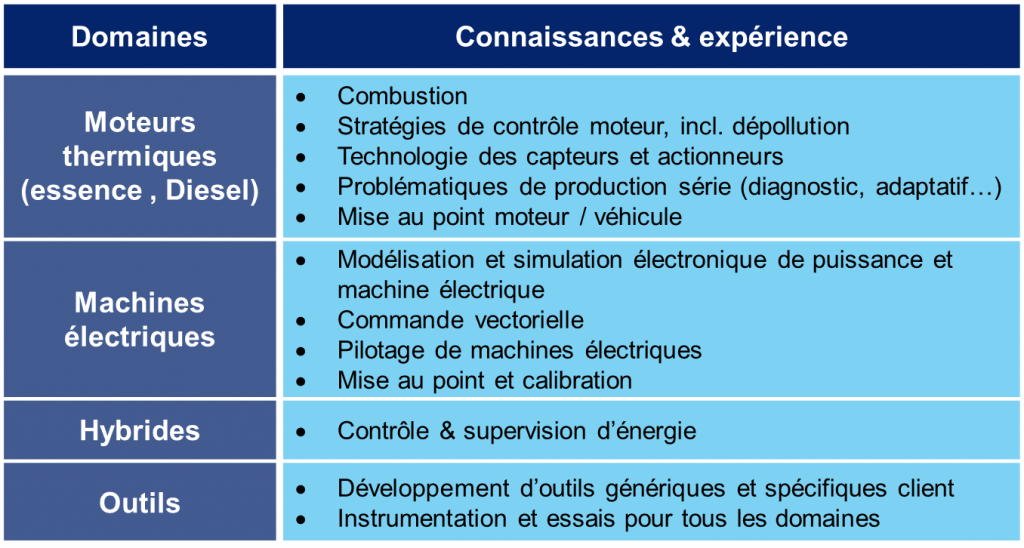
\includegraphics[scale=0.3]{images/domaines}\\
  \end{center}
\end{frame}

%%%%%%%%%%%%%%%%%%%%%%%%%%%%%%%%%%%%%%%%%%%%%%%%%%%%%%
%%%%%%%%%%%%%%%%%%%%%%%%%%%%%%%%%%%%%%%%%%%%%%%%%%%%%%
\section{\scshape Objectifs}
\begin{frame}{\vspace{-17pt}\\
\includegraphics[scale=0.34]{images/orianne}}
  \begin{center}
	\onslide<1->{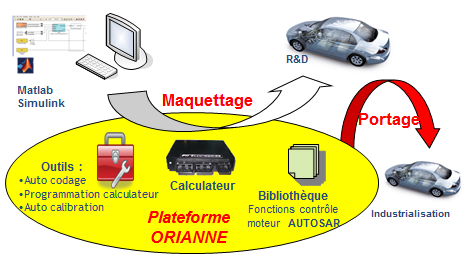
\includegraphics[scale=0.6]{images/Orianne}}
	\vfill
	\onslide<2->{
	  \begin{tabular}[h]{m{110pt}m{53pt}m{125pt}}
	  
\includegraphics[scale=0.05]{images/matlab_simulink_cross} &
	  
\includegraphics[scale=2.5]{images/rightarrow} &
	  
\includegraphics[scale=0.1]{images/qgen} \\
	  \end{tabular}
	}
  \end{center}
\end{frame}

\begin{frame}{\vspace{-17pt}\\
\includegraphics[scale=0.04]{images/qgen}}
  \begin{center}
	Générateur de code embarqué C/Ada depuis Matlab Simulink\\
	\vfill
	
\includegraphics[scale=0.2]{images/adacore.png}\\
	\vfill
	\begin{block}{Avantages}{}
	  \begin{itemize}
		\item Prix
		\item Maîtrise
	  \end{itemize}
	\end{block}
  \end{center}
\end{frame}

\begin{frame}{{\bf C}ontroller {\bf A}rea {\bf N}etwork}
  \begin{center}
	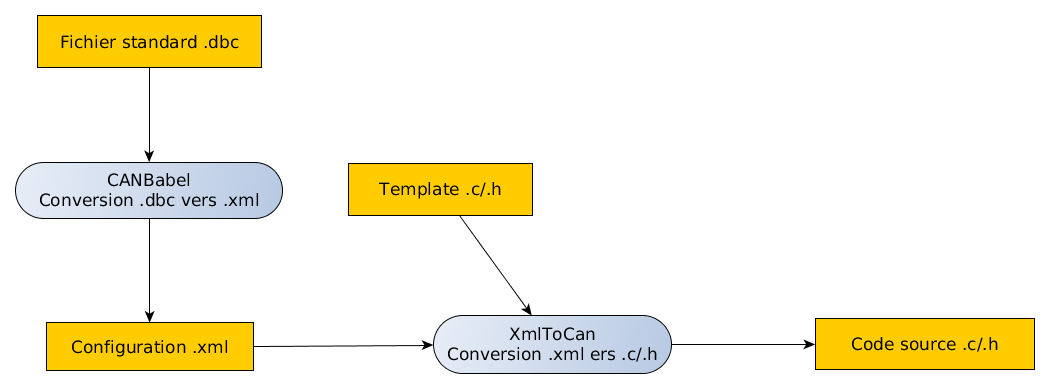
\includegraphics[scale=0.28]{images/dbctocan}\\
	\vfill
	Processus de convertion des fichiers .dbc vers du code source C
  \end{center}
\end{frame}

\begin{frame}{Objectifs}
  \begin{block}{Court terme}{}
	\begin{itemize}
	  \item Outil stable
	  \item Certification
	  \item IHM fonctionnelle
	\end{itemize}
  \end{block}
  \begin{block}{Long terme}{}
	\begin{itemize}
	  \item Automatisation complète
	  \item Généricité
	  \item Maintenabilité
	\end{itemize}
  \end{block}
\end{frame}

%%%%%%%%%%%%%%%%%%%%%%%%%%%%%%%%%%%%%%%%%%%%%%%%%%%%%%
%%%%%%%%%%%%%%%%%%%%%%%%%%%%%%%%%%%%%%%%%%%%%%%%%%%%%%
\section{\scshape Démarche}
\begin{frame}{Etude du code RTW/EC}
  \begin{itemize}
	\item Code généré par Simulink
	\item Analyseur OCLint
	\item Génération de rapport (python)
  \end{itemize}
\end{frame}

\begin{frame}{Etude de QGen}
  \begin{itemize}
	\item Reprise de l'étude
	\item Adaptation des modèles
	  \only<2->{\begin{itemize}
		\item Blocks compatibles
		\item Retours de bugs
	  \end{itemize}}
	\item Génération de code
	  \only<3->{\begin{itemize}
		\item Génération des modules
		\item Lien entre ces modules
		\item Analyse statique
	  \end{itemize}}
  \end{itemize}
\end{frame}

\begin{frame}{Intégration à Orianne}{Automatisation}
  \vfill
  Base de code générée par QGen
  \vfill
  \begin{itemize}
	\item Appel des composants
	\item Makefile
	\item Paramètres
  \end{itemize}
  \vfill
\end{frame}

\begin{frame}{Configuration CAN}
  \begin{itemize}
	\item Étude du code existant
	\item \og Refactoring \fg{} et optimization
	\item Adaptation des templates
  \end{itemize}
\end{frame}

%%%%%%%%%%%%%%%%%%%%%%%%%%%%%%%%%%%%%%%%%%%%%%%%%%%%%%
%%%%%%%%%%%%%%%%%%%%%%%%%%%%%%%%%%%%%%%%%%%%%%%%%%%%%%
\section{\scshape Etat d'avancement}
\begin{frame}{RTW/EC analysé}
  \begin{itemize}
	\item Définition des seuils de violation
	\item Génération de rapports
	\item Aggrégation des métriques
  \end{itemize}
\end{frame}

\begin{frame}{Génération via QGen}
  \begin{itemize}
	\item Code généré pour tous les modules (perl)
	\item Code analysé avec OCLint
  \end{itemize}
\end{frame}

\begin{frame}{Intégration à Orianne}
  \begin{itemize}
	\item \og glue \fg{} entre les composants
	\item Échanges de paramètres entre modules
  \end{itemize}
\end{frame}

\begin{frame}{{\bf C}ontroller {\bf A}rea {\bf N}etwork}
  \begin{itemize}
	\item Étude des problèmes de génération
	\item Intégration du nouveau template
  \end{itemize}
\end{frame}


%%%%%%%%%%%%%%%%%%%%%%%%%%%%%%%%%%%%%%%%%%%%%%%%%%%%%%
%%%%%%%%%%%%%%%%%%%%%%%%%%%%%%%%%%%%%%%%%%%%%%%%%%%%%%
\section*{}

\begin{frame}
\title{Intégration d'un générateur de code embarqué dans une plateforme de
  prototypage rapide de fonctions de contrôle moteur}
%\subtitle{SUBTITLE}
\author{
  \vspace{-15px}\\
  Mathieu {\sc Soum}\\
  {\footnotesize
	Université Paul Sabatier\\
	\vspace{-3px}
    Master 2 -- Développement Logiciel
  }
  \vspace{5px}\\
  {\small Stage réalisé chez Aboard Engineering}\\
  {\scriptsize
	Maître de stage : Sébastien {\sc Riche}\\
	\vspace{-3px}
	Tutrice universitaire : Isabelle {\sc Ferrané}
  }
  \vspace{-17px}
}
\date{
	{
	  \begin{tabular}{m{90pt}m{105pt}m{85pt}}
		
\includegraphics[scale=0.20]{images/aboard} &
		
\includegraphics[scale=0.3]{images/mdl} &
		
\includegraphics[scale=0.25]{images/ups} \\
	  \end{tabular}
	  %
\includegraphics[scale=0.4]{images/aboard}\hspace{75px}
\includegraphics[scale=0.37]{images/ups}
	}
	\\
	\vspace{5px}
	Année universitaire 2013 - 2014
}
\titlepage
\end{frame}
  
\end{document}
